% compile with: pdflatex -shell-escape filename.tex
\documentclass[crop,tikz,convert=pdf2svg]{standalone}
\usepackage{tikz}
\usetikzlibrary{arrows.meta}
\usetikzlibrary{bending}
\usetikzlibrary{backgrounds}
\usetikzlibrary{calc}
\usetikzlibrary{decorations.pathreplacing}
\usetikzlibrary{matrix}
\usetikzlibrary{positioning}

\tikzset{
  ncbar angle/.initial=90,
  ncbar/.style={
    to path=(\tikztostart)
    -- ($(\tikztostart)!#1!\pgfkeysvalueof{/tikz/ncbar angle}:(\tikztotarget)$)
    -- ($(\tikztotarget)!($(\tikztostart)!#1!\pgfkeysvalueof{/tikz/ncbar angle}:(\tikztotarget)$)!\pgfkeysvalueof{/tikz/ncbar angle}:(\tikztostart)$)
    -- (\tikztotarget)
  },
  ncbar/.default=0.5cm,
}

\tikzset{
  bracket/.style={ncbar=-0.25cm},
  block_arrow/.style={-{Stealth[length=10pt]}, color=blue, thick},
  block_bunch/.style={color=blue, thick},
}

\begin{document}

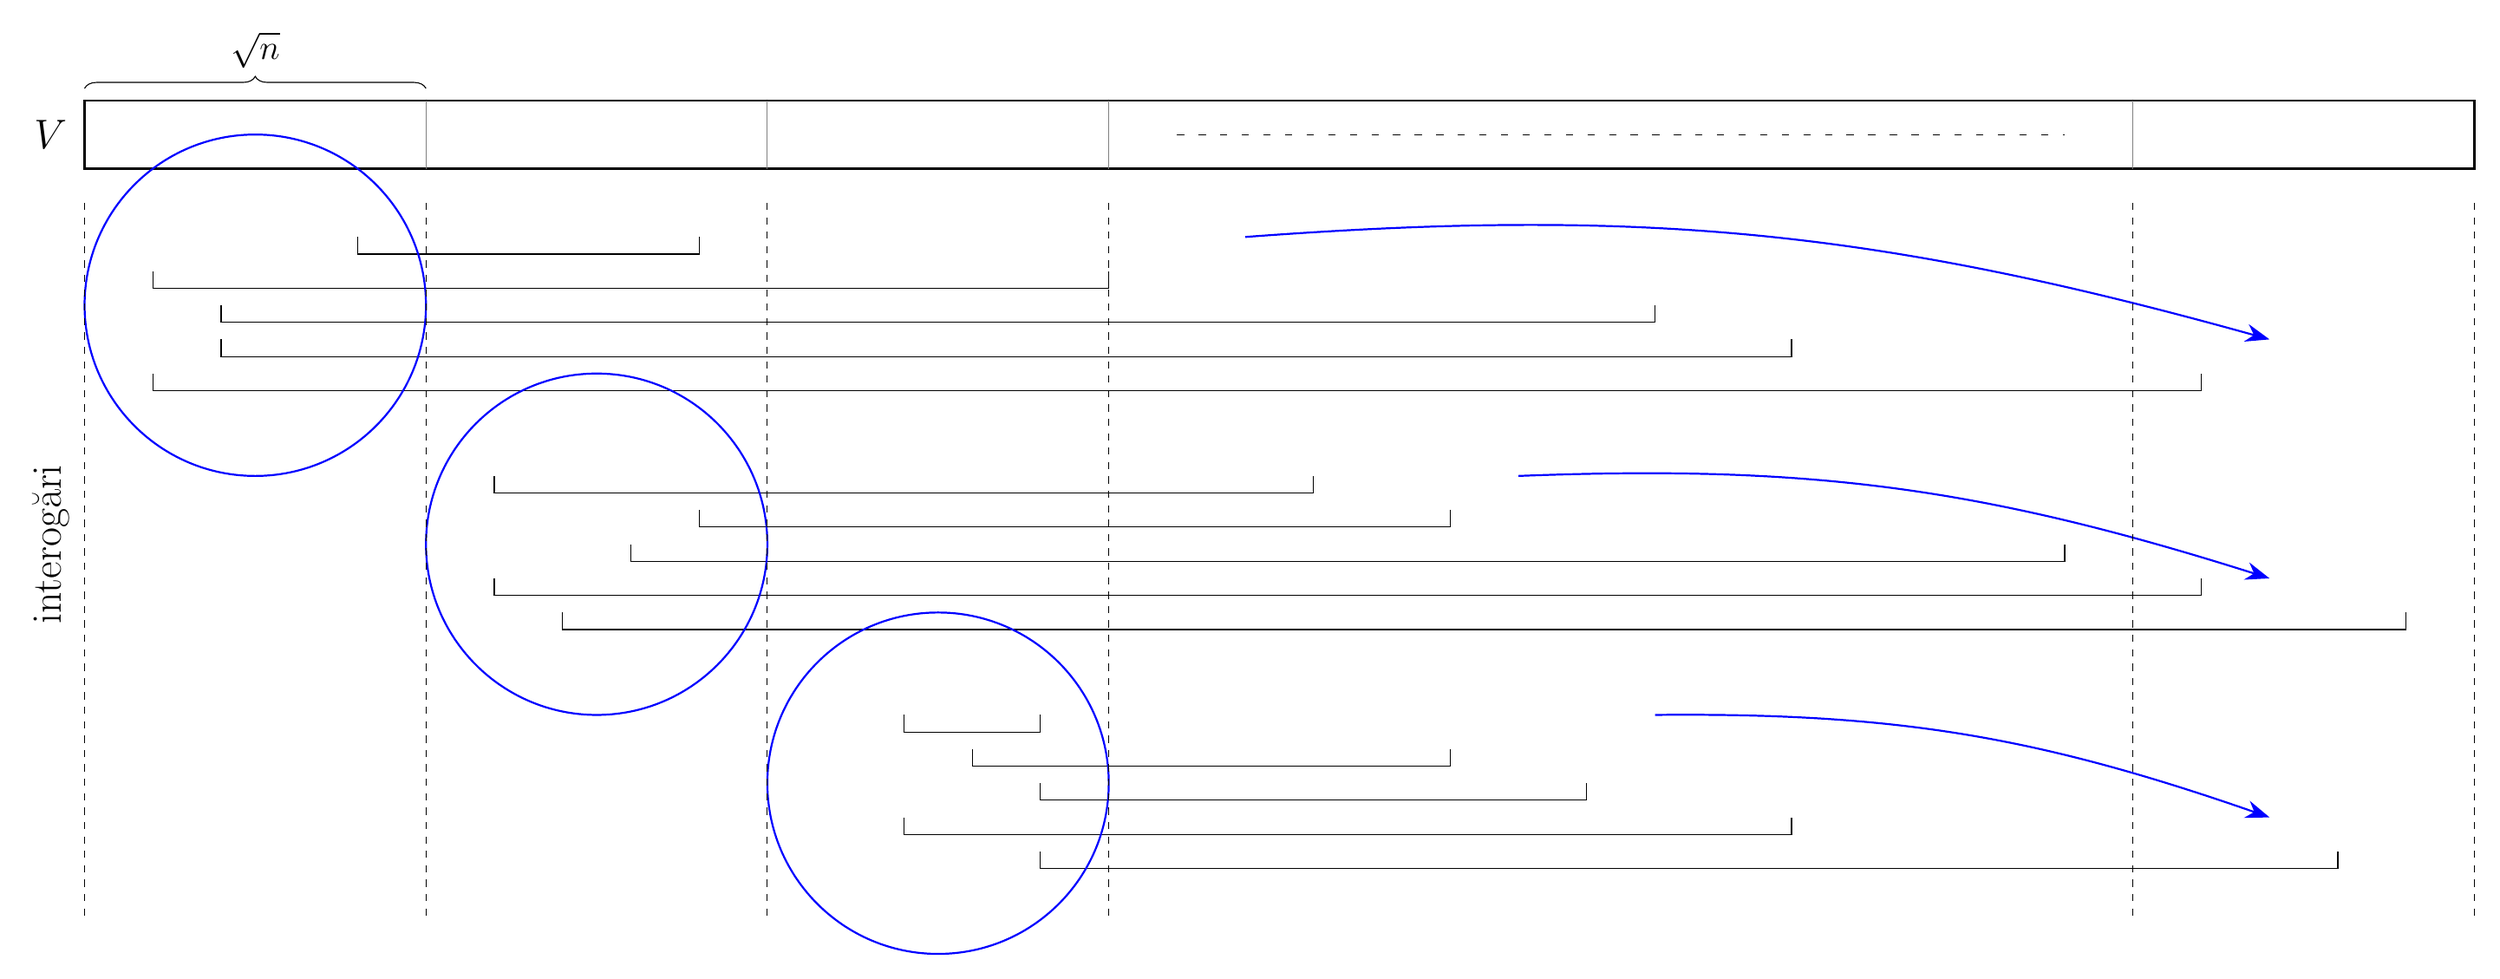
\begin{tikzpicture}
  % V and its blocks
  \draw [draw=black,thick] (0, 0) rectangle (35, -1);
  \draw [gray] (5, 0) -- (5, -1);
  \draw [gray] (10, 0) -- (10, -1);
  \draw [gray] (15, 0) -- (15, -1);
  \draw [gray] (30, 0) -- (30, -1);
  \draw [loosely dashed] (16, -0.5) -- (29, -0.5);

  % Labels
  \node at (-0.5, -0.5) {\LARGE $V$};
  \node at (-0.5, -6.5) [rotate=90] {\LARGE interogări};
  \draw [
    decorate,
	  decoration = {brace, raise=5pt, amplitude=5pt, }
  ] (0, 0) -- (5, 0)
  node [pos=0.5,above=10pt] {\Large $\sqrt{n}$};

  % Queries in first block
  \draw (4, -2) to [bracket] (9, -2);
  \draw (1, -2.5) to [bracket] (15, -2.5);
  \draw (2, -3) to [bracket] (23, -3);
  \draw (2, -3.5) to [bracket] (25, -3.5);
  \draw (1, -4) to [bracket] (31, -4);
  \draw[block_bunch](2.5, -3) circle (2.5);
  \draw (17, -2) edge[block_arrow,bend left=10] (32, -3.5);

  % Queries in second block
  \draw (6, -5.5) to [bracket] (18, -5.5);
  \draw (9, -6) to [bracket] (20, -6);
  \draw (8, -6.5) to [bracket] (29, -6.5);
  \draw (6, -7) to [bracket] (31, -7);
  \draw (7, -7.5) to [bracket] (34, -7.5);
  \draw[block_bunch](7.5, -6.5) circle (2.5);
  \draw (21, -5.5) edge[block_arrow,bend left=10] (32, -7);

  % Queries in third block
  \draw (12, -9) to [bracket] (14, -9);
  \draw (13, -9.5) to [bracket] (20, -9.5);
  \draw (14, -10) to [bracket] (22, -10);
  \draw (12, -10.5) to [bracket] (25, -10.5);
  \draw (14, -11) to [bracket] (33, -11);
  \draw[block_bunch](12.5, -10) circle (2.5);
  \draw (23, -9) edge[block_arrow,bend left=10] (32, -10.5);

  \draw [dashed] (0, -1.5) -- (0, -12);
  \draw [dashed] (5, -1.5) -- (5, -12);
  \draw [dashed] (10, -1.5) -- (10, -12);
  \draw [dashed] (15, -1.5) -- (15, -12);
  \draw [dashed] (30, -1.5) -- (30, -12);
  \draw [dashed] (35, -1.5) -- (35, -12);
\end{tikzpicture}

\end{document}
